\documentclass[tikz,dvipdfmx,dvipsnames]{standalone}

\usepackage{amsmath, amssymb, amsthm, mathrsfs, amsfonts, dsfont}
\usepackage{bbm}
\usepackage{bm}
\usepackage{physics}
\usepackage{ifthen}
\usepackage{setspace}
\usepackage{mathtools}

\newcommand{\defeq}{\coloneqq}

\newcommand{\red}[1]{\textcolor{red}{#1}}
\newcommand{\blue}[1]{\textcolor{blue}{#1}}
\newcommand{\cyan}[1]{\textcolor{cyan}{#1}}
\newcommand{\gray}[1]{\textcolor{gray}{#1}}
\newcommand{\green}[1]{\textcolor{green}{#1}}
\newcommand{\brown}[1]{\textcolor{brown}{#1}}
\newcommand{\black}[1]{\textcolor{black}{#1}}
\newcommand{\orange}[1]{\textcolor{orange}{#1}}
\newcommand{\purple}[1]{\textcolor{purple}{#1}}
\newcommand{\yellow}[1]{\textcolor{yellow}{#1}}
\newcommand{\Magenta}[1]{\textcolor{Magenta}{#1}}
\newcommand{\RoyalBlue}[1]{\textcolor{RoyalBlue}{#1}}
\newcommand{\RubineRed}[1]{\textcolor{RubineRed}{#1}}
\newcommand{\ForestGreen}[1]{\textcolor{ForestGreen}{#1}}
\newcommand{\YellowOrange}[1]{\textcolor{YellowOrange}{#1}}
\newcommand{\WildStrawberry}[1]{\textcolor{WildStrawberry}{#1}}

\definecolor{cA}{HTML}{0072BD}
\definecolor{cB}{HTML}{EDB120}
\definecolor{cC}{HTML}{77AC30}
\definecolor{cD}{HTML}{D95319}

\usetikzlibrary{calc,matrix,math}

\begin{document}
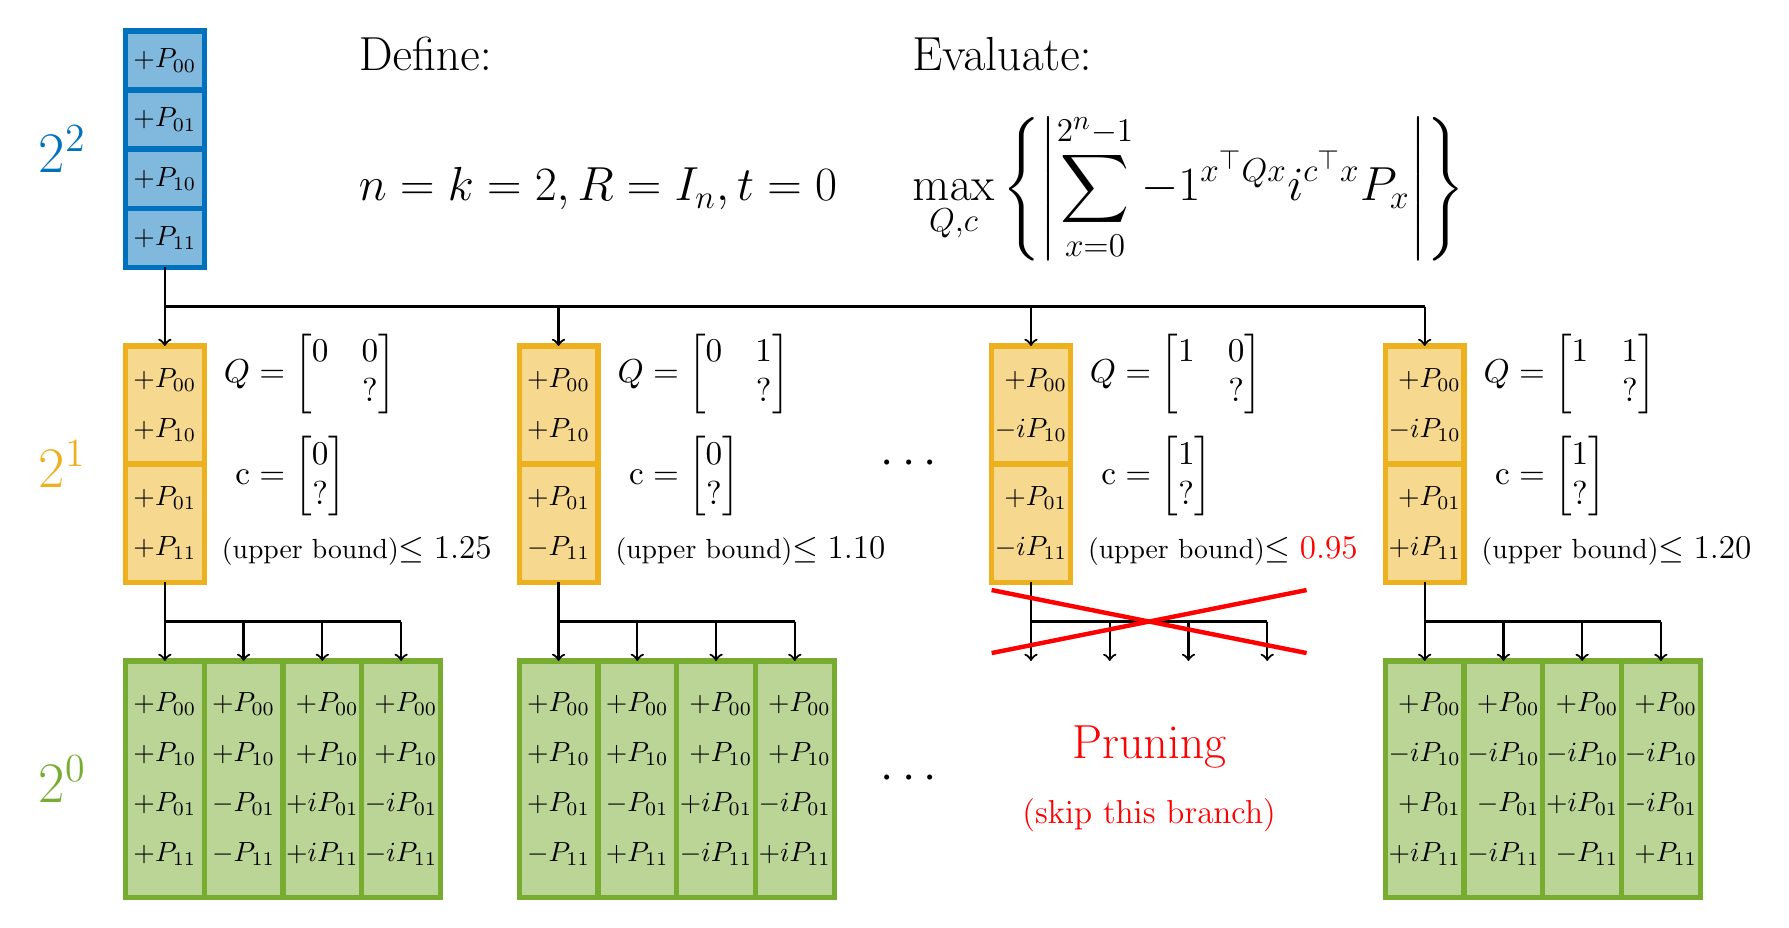
\begin{tikzpicture}[
        myBlock1/.style={draw=cA,fill=cA!50,line width=1.9pt},
        myBlock2/.style={draw=cB,fill=cB!50,line width=1.9pt},
        myBlock3/.style={draw=cC,fill=cC!50,line width=1.9pt},
        myNode/.style={align=right,midway},
    ]
    \foreach \i/\bit in {0/00,1/01,2/10,3/11}{
    \renewcommand{\baselinestretch}{1.5}
    \draw[myBlock1](0,-3/4*\i) rectangle (1,-3/4*\i-0.75) node[myNode] {$+P_{\bit}$};
    \renewcommand{\baselinestretch}{1.0}
    }

    \foreach \pos/\a/\b/\c/\d/\x/\y/\z/\thres/\thresColor in {
            0/+/+/+/+/0/0/0/1.25/\black,
            5/+/+/+/-/0/0/1/1.10/\black,
            11/+/+/-i/-i/1/1/0/0.95/\red,
            16/+/+/-i/+i/1/1/1/1.20/\black
        }{
            \renewcommand{\baselinestretch}{1.5}
            \draw[myBlock2](\pos,-4) rectangle (\pos+1,-5.5) node[myNode] {$\a P_{00}$\\$\c P_{10}$};
            \draw[myBlock2](\pos,-5.5) rectangle (\pos+1,-7) node[myNode] {$\b P_{01}$\\$\d P_{11}$};
            \renewcommand{\baselinestretch}{1.0}
            \node[anchor=north west,scale=1.2] at (\pos+1.1,-3.7) {$Q=\mqty[\y&\z\\&?]$};
            \node[anchor=north west,scale=1.2] at (\pos+1.1,-5.0) {$\phantom{Q}\makebox[0pt][r]{c}=\mqty[\x\\?]$};
            \node[anchor=north west] at (\pos+1.1,-6.3) {(upper bound)\\\large{$\leq \thresColor{\thres}$}};
        }

    \foreach \i/\x/\a/\b/\c/\d in {
            0/0/ +/ +/ +/ +/,
            1/1/ +/ -/ +/ -/,
            2/2/ +/+i/ +/+i/,
            3/3/ +/-i/ +/-i/,
            4/5/ +/ +/ +/ -/,
            5/6/ +/ -/ +/ +/,
            6/7/ +/+i/ +/-i/,
            7/8/ +/-i/ +/+i/,
            28/16/ +/ +/-i/+i/,
            29/17/ +/ -/-i/-i/,
            30/18/ +/+i/-i/ -/,
            31/19/ +/-i/-i/ +/
        }{
            \renewcommand{\baselinestretch}{1.5}
            \draw[myBlock3] (\x,-8) rectangle (\x+1,-11)
            node[myNode] {$\a P_{00}$\\$\c P_{10}$\\$\b P_{01}$\\$\d P_{11}$};
            \renewcommand{\baselinestretch}{1.0}
            % \node[font=\large] at (\x+0.5,-11.5) {$\i$};
        }

    \newcommand{\Arrows}[3]{
        \begin{scope}[xshift=#1.0cm, yshift=-#2.0cm]
            \draw[thick,->] (0.5,-0.0) -- (0.5,-1.0); % node[xshift=8,yshift=7] {$+$};
            \draw[thick,->] (1.5,-0.5) -- (1.5,-1.0); % node[xshift=8,yshift=7] {$-$};
            \draw[thick,->] (2.5,-0.5) -- (2.5,-1.0); % node[xshift=8,yshift=7] {$+i$};
            \draw[thick,->] (3.5,-0.5) -- (3.5,-1.0); % node[xshift=8,yshift=7] {$-i$};
            \draw[thick,  ] (0.5,-0.5) -- (3.5,-0.5);
        \end{scope}}
    \draw[thick,->] (0.5 ,-3.0) -- (0.5 ,-4.0);
    \draw[thick,->] (5.5 ,-3.5) -- (5.5 ,-4.0);
    \draw[thick,->] (11.5,-3.5) -- (11.5,-4.0);
    \draw[thick,->] (16.5,-3.5) -- (16.5,-4.0);
    \draw[thick,  ] (0.5 ,-3.5) -- (16.5,-3.5);
    \Arrows{0}{7}{1}
    \Arrows{5}{7}{1}
    \Arrows{11}{7}{1}
    \Arrows{16}{7}{1}

    \draw[ultra thick,red] (11,-7.1) -- (15,-7.9);
    \draw[ultra thick,red] (11,-7.9) -- (15,-7.1);
    \node[align=center,red] at (13,-9.5) {\LARGE{Pruning}\\[1em]\large{(skip this branch)}};

    \node[anchor=center,font=\LARGE] at (10,-5.5) {$\cdots$};
    \node[anchor=center,font=\LARGE] at (10,-9.5) {$\cdots$};

    \node[font=\LARGE,cA,scale=1.2] at (-0.8,-1.5) {$2^2$};
    \node[font=\LARGE,cB,scale=1.2] at (-0.8,-5.5) {$2^1$};
    \node[font=\LARGE,cC,scale=1.2] at (-0.8,-9.5) {$2^0$};

    \node[font=\LARGE,align=left] at (6,-1.5) {
        Define:\\[0.9em]
        $n=k=2, R=I_n, t=0 \vphantom{{\displaystyle \sum_{x=0}^{2^n-1}}}$
    };
    \node[font=\LARGE,align=left] at (13.5,-1.5) {
    Evaluate: \\[0.9em]
    ${\displaystyle \max_{Q,c}\qty{\abs{\sum_{x=0}^{2^n-1} -1^{x^\top Q x} i^{c^\top x} P_x}}}$
    };

\end{tikzpicture}
\end{document}
